Cada sección transversal vertical del siguiente prisma triangular (figura \ref{fig:pitagoras3D_pris_01}) es un triángulo isósceles.
\begin{figure}[H]
    \begin{center}
        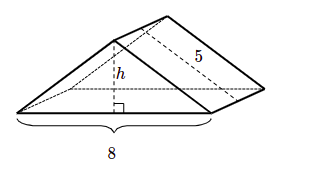
\includegraphics[width=0.5\textwidth]{../images/pitagoras3D_pris_01.png}
    \end{center}
    \caption{}
    \label{fig:pitagoras3D_pris_01}
\end{figure}
\textbf{¿Cuál es la altura $h$ del prisma triangular?}\\
\textit{Redondea tu respuesta a la décima más cercana.}